% PCCSL 507 Machine Learning Lab - Experiment 1 (NumPy only, housing.csv)
\documentclass[11pt,twoside]{article}

\usepackage[paper=letterpaper,top=0.7in,bottom=0.63in,left=0.75in,right=0.75in,headheight=24pt,headsep=0.14in,footskip=0.38in]{geometry}

\usepackage[T1]{fontenc}
\usepackage{mathptmx} % Times clone
\usepackage{xcolor}
\definecolor{primary}{HTML}{1F3864}
\definecolor{greytext}{HTML}{555555}
\definecolor{gridgrey}{HTML}{999999}
\usepackage{fancyhdr}
\usepackage{array}
\usepackage{colortbl}
\usepackage{parskip}
\setlength{\parindent}{0pt}
\setlength{\parskip}{4pt}
\setlength{\abovedisplayskip}{4pt}
\setlength{\belowdisplayskip}{4pt}
\setlength{\abovedisplayshortskip}{2pt}
\setlength{\belowdisplayshortskip}{2pt}
\usepackage{graphicx}
\usepackage{listings}
\lstset{basicstyle=\footnotesize\ttfamily, breaklines=true, frame=single, showstringspaces=false}

\pagestyle{fancy}
\fancyhf{}
\fancyhead[C]{\textcolor{primary}{\textbf{\small PCCSL 507 Machine Learning Laboratory Record}}}
\renewcommand{\headrulewidth}{0.75pt}
\renewcommand{\headrule}{\hbox to\headwidth{\color{primary}\leaders\hrule height \headrulewidth\hfill}}
\fancyfoot[C]{\footnotesize DEPARTMENT OF CSE \hfill CAPE COLLEGE OF ENGINEERING ALAPPUZHA \hfill Page No. \thepage}
\renewcommand{\footrulewidth}{0pt}

\newcommand{\expheading}[1]{{\fontsize{14}{17}\selectfont\textbf{#1}\par}}
\newcommand{\fullrule}{\noindent\rule{\textwidth}{0.6pt}\par}

\begin{document}
\sloppy

% ================= COVER (p1, right) =================
\begin{center}
\vspace*{38pt}
{\fontsize{15}{18}\selectfont\textcolor{primary}{\textbf{CAPE COLLEGE OF ENGINEERING ALAPPUZHA}}}\par
\vspace{10pt}
{\fontsize{11}{14}\selectfont\textcolor{greytext}{Department of \underline{\hspace{4.5cm}}}}\par
\vspace{28pt}
{\color{primary}\rule{\textwidth}{0.75pt}}\par
\vspace{6pt}
{\fontsize{20}{24}\selectfont\textcolor{primary}{\textbf{PCCSL 507 MACHINE LEARNING LAB}}}\par
\vspace{6pt}
{\color{primary}\rule{\textwidth}{0.75pt}}\par
\vspace{10pt}
{\fontsize{15}{18}\selectfont\textbf{LABORATORY RECORD}}\par
\vspace{28pt}
{\fontsize{11}{14}\selectfont Submitted by}\par
\vspace{8pt}
\end{center}

{\fontsize{11}{16}\selectfont
\begin{center}
\renewcommand{\arraystretch}{1.6}
\begin{tabular}{@{}p{3.6cm}@{\hspace{0.2cm}:\hspace{0.3cm}}l@{}}
Name & \underline{\hspace{6.2cm}} \\
Reg.\ No. & \underline{\hspace{6.2cm}} \\
Programme & \underline{\hspace{6.2cm}} \\
Semester / Year & \underline{\hspace{6.2cm}} \\
Academic Year & \underline{\hspace{6.2cm}} \\
Faculty In-Charge & \underline{\hspace{6.2cm}} \\
\end{tabular}
\end{center}
\vspace{14pt}
\begin{center}
\begin{tabular}{@{}l@{\hspace{0.2cm}:\hspace{0.3cm}}l@{\hspace{1.0cm}}l@{\hspace{0.2cm}:\hspace{0.3cm}}l@{}}
Signature & \underline{\hspace{2.9cm}} & Date & \underline{\hspace{2.9cm}} \\
\end{tabular}
\end{center}
}

\newpage
\null\thispagestyle{empty}\newpage % p2 blank (double-side parity)

% ================= INDEX (p3, right) =================
\begin{center}
{\fontsize{16}{19}\selectfont\textcolor{primary}{\textbf{INDEX}}}\par
\vspace{8pt}
\end{center}

\setlength{\tabcolsep}{4pt}
\arrayrulecolor{gridgrey}
\setlength{\arrayrulewidth}{0.5pt}
\noindent
\begin{tabular}{|>{\centering\arraybackslash}p{0.44in}|>{\centering\arraybackslash}p{3.34in}|>{\centering\arraybackslash}p{0.94in}|>{\centering\arraybackslash}p{0.75in}|>{\centering\arraybackslash}p{0.86in}|}
\hline
\rowcolor{primary}
\textcolor{white}{\textbf{\small Sl.\ No.}} & \textcolor{white}{\textbf{\small Title of the Experiment}} & \textcolor{white}{\textbf{\small Date}} & \textcolor{white}{\textbf{\small Page No.}} & \textcolor{white}{\textbf{\small Signature}} \\
\hline
1 & Simple Linear Regression (Least Squares \& Gradient Descent) & & 5 & \\[14pt] \hline
2  &  &  &  &  \\[14pt] \hline
3  &  &  &  &  \\[14pt] \hline
4  &  &  &  &  \\[14pt] \hline
5  &  &  &  &  \\[14pt] \hline
6  &  &  &  &  \\[14pt] \hline
7  &  &  &  &  \\[14pt] \hline
8  &  &  &  &  \\[14pt] \hline
9  &  &  &  &  \\[14pt] \hline
10 &  &  &  &  \\[14pt] \hline
11 &  &  &  &  \\[14pt] \hline
12 &  &  &  &  \\[14pt] \hline
13 &  &  &  &  \\[14pt] \hline
14 &  &  &  &  \\[14pt] \hline
15 &  &  &  &  \\[14pt] \hline
\end{tabular}

\newpage
\null\thispagestyle{empty}\newpage % p4 blank (double-side parity)

% Sheet-local tightening so Title/Theory fits one right-side page
{\setlength{\parskip}{1pt}\setlength{\abovedisplayskip}{2pt}\setlength{\belowdisplayskip}{2pt}
\begin{center}
\expheading{EXPERIMENT NO. 1}
\end{center}
\vspace{2pt}

\noindent\textbf{Date:} \underline{\hspace{2.6cm}} \hfill \textbf{Page No.:} \underline{\hspace{2.6cm}}\par
\vspace{6pt}

\expheading{TITLE}
\vspace{4pt}
\noindent Simple Linear Regression using Least Squares and Gradient Descent\par
\vspace{4pt}

\expheading{OBJECTIVE}
\vspace{2pt}
\fullrule
\vspace{4pt}
\noindent To implement simple linear regression on housing.csv by least squares and gradient descent (X=TotalRooms, Y=MedHouseVal), and evaluate it with MSE, R-squared and the regression-line plot. \par
\vspace{4pt}

\expheading{AIM}
\vspace{4pt}
\noindent To predict MedHouseVal from TotalRooms with SLR (least squares and gradient descent, $\alpha=0.01$, 100 epochs), and assess the fit using MSE and $R^2$. \par
\vspace{4pt}

\expheading{THEORY}
\vspace{4pt}
Regression equation:
\[\hat{Y}=mX+b\]
Least-squares estimates:
\[m=\frac{\sum_{i=1}^{n}(X_i-\bar{X})(Y_i-\bar{Y})}{\sum_{i=1}^{n}(X_i-\bar{X})^2}\qquad b=\bar{Y}-m\bar{X}\]
Mean Squared Error cost:
\[J(m,c)=\frac{1}{n}\sum_{i=1}^{n}(Y_i-\hat{Y}_i)^2\]
Gradients:
\[\frac{\partial J}{\partial m}=-\frac{2}{n}\sum_{i=1}^{n}X_i(Y_i-\hat{Y}_i)\qquad \frac{\partial J}{\partial b}=-\frac{2}{n}\sum_{i=1}^{n}(Y_i-\hat{Y}_i)\]
Gradient descent updates:
\[m:=m-\alpha\frac{\partial J}{\partial m}\qquad b:=b-\alpha\frac{\partial J}{\partial b}\]
Goodness of fit:
\[\mathrm{MSE}=\frac{1}{n}\sum_{i=1}^{n}(Y_i-\hat{Y}_i)^2\qquad R^2=1-\frac{\sum_{i=1}^{n}(Y_i-\hat{Y}_i)^2}{\sum_{i=1}^{n}(Y_i-\bar{Y})^2}\]
\vspace{4pt}

\expheading{PROCEDURE}
\vspace{4pt}
\noindent A) Least Squares: load housing.csv; take X=TotalRooms, Y=MedHouseVal; inspect missing, duplicate and invalid values; compute slope $m$ and intercept $b$ by least squares; form $\hat{Y}=mX+b$; predict the test set; report MSE and $R^2$; plot data points with the regression line.\par
\noindent B) Gradient Descent: load housing.csv (X=TotalRooms, Y=MedHouseVal); clean the data; 80/20 split; standardize X with train mean/std; init $m=c=0$; set $\alpha=0.01$, epochs=100; iterate predict $\rightarrow$ cost $J$ $\rightarrow$ gradients $\rightarrow$ update $m,b$; plot cost vs epochs; predict test data with final $m,b$; report MSE and $R^2$.\par
\vspace{4pt}

\expheading{DATASET DESCRIPTION}
\vspace{4pt}
\noindent Dataset Name: California Housing (housing.csv)\par
\noindent Source: Public census CSV file; prepared with NumPy only\par
\noindent Number of Samples: 20640 usable (0 missing, 118 duplicates, 0 invalid) \hspace{0.3cm} Number of Features: 1 (TotalRooms)\par
\noindent Target / Class: MedHouseVal $-$ median house value in units of \$100{,}000\par
\noindent Description: Train 16512 / test 4128 (80/20, seed 42); feature standardized. \par
\vspace{4pt}
} % end sheet-local tightening

\newpage
\expheading{PROGRAM}
\vspace{6pt}

\begin{lstlisting}
import csv
import numpy as np
import matplotlib
matplotlib.use("Agg")
import matplotlib.pyplot as plt


rooms, prices, miss = [], [], 0
with open("housing.csv", newline="") as f:
    for r in csv.DictReader(f):
        try:
            rooms.append(float(r["total_rooms"]))
            prices.append(float(r["median_house_value"]))
        except (ValueError, KeyError):
            miss += 1
X = np.array(rooms)
y = np.array(prices) / 1e5
print("Usable:", len(X), " Missing:", miss)


rng = np.random.default_rng(42)
order = np.arange(len(X))
rng.shuffle(order)
n_train = int(0.8 * len(X))
X_train, X_test = X[order[:n_train]], X[order[n_train:]]
y_train, y_test = y[order[:n_train]], y[order[n_train:]]
print("Train:", len(X_train), " Test:", len(X_test))


x_bar = X_train.mean()
y_bar = y_train.mean()
m = ((X_train - x_bar) * (y_train - y_bar)).sum()
m = m / ((X_train - x_bar) ** 2).sum()
b = y_bar - m * x_bar
print(f"LS slope m = {m:.6f}")
print(f"LS intercept b = {b:.4f}")

y_pred = m * X_test + b
mse = ((y_test - y_pred) ** 2).mean()
r2 = 1 - ((y_test - y_pred) ** 2).sum() / ((y_test - y_test.mean()) ** 2).sum()
print(f"LS: MSE={mse:.4f} R2={r2:.4f} RMSE={np.sqrt(mse):.4f}")

plt.figure(figsize=(7, 4.5))
plt.scatter(X_test, y_test, s=6, alpha=0.25, label="Test data")
xs = np.linspace(0, float(np.percentile(X, 99.5)), 200)
plt.plot(xs, m * xs + b, linewidth=2, label="Least Squares line")
plt.xlabel("TotalRooms (X)")
plt.ylabel("MedHouseVal ($100k) (Y)")
plt.title("SLR: TotalRooms vs Median House Value")
plt.legend()
plt.tight_layout()
plt.savefig("exp1_ls.png", dpi=150)

mu = X_train.mean()
sg = X_train.std()
Xs_train = (X_train - mu) / sg
m, b = 0.0, 0.0
n = len(Xs_train)
costs = []
for epoch in range(100):
    y_hat = m * Xs_train + b
    err = y_train - y_hat
    J = (err ** 2).mean()
    costs.append(float(J))
    dm = (-2 / n) * (Xs_train * err).sum()
    db = (-2 / n) * err.sum()
    m = m - 0.01 * dm
    b = b - 0.01 * db
m_gd = m / sg
b_gd = b - m * mu / sg
print(f"GD slope m = {m_gd:.6f}")
print(f"GD intercept b = {b_gd:.4f}")
print(f"GD cost first={costs[0]:.4f} last={costs[-1]:.4f}")
y_pred = m_gd * X_test + b_gd
mse = ((y_test - y_pred) ** 2).mean()
r2 = 1 - ((y_test - y_pred) ** 2).sum() / ((y_test - y_test.mean()) ** 2).sum()
print(f"GD: MSE={mse:.4f} R2={r2:.4f} RMSE={np.sqrt(mse):.4f}")
plt.figure(figsize=(6, 3.8))
plt.plot(range(1, 101), costs)
plt.xlabel("Epoch")
plt.ylabel("Cost J (MSE)")
plt.title("Gradient Descent: Cost vs Epochs")
plt.tight_layout()
plt.savefig("exp1_cost.png", dpi=150)
\end{lstlisting}

\newpage
\expheading{OUTPUT}
\vspace{2pt}
\noindent\rule{\textwidth}{0.5pt}\par
\vspace{4pt}
\begin{verbatim}
Usable: 20640  Missing: 0
Train: 16512  Test: 4128
LS slope m = 0.000072
LS intercept b = 1.8840
LS: MSE=1.3236 R2=0.0167 RMSE=1.1505
GD slope m = 0.000062
GD intercept b = 1.6341
GD cost first=5.6208 last=1.3827
GD: MSE=1.3885 R2=-0.0315 RMSE=1.1784
\end{verbatim}
\vspace{4pt}

\begin{center}
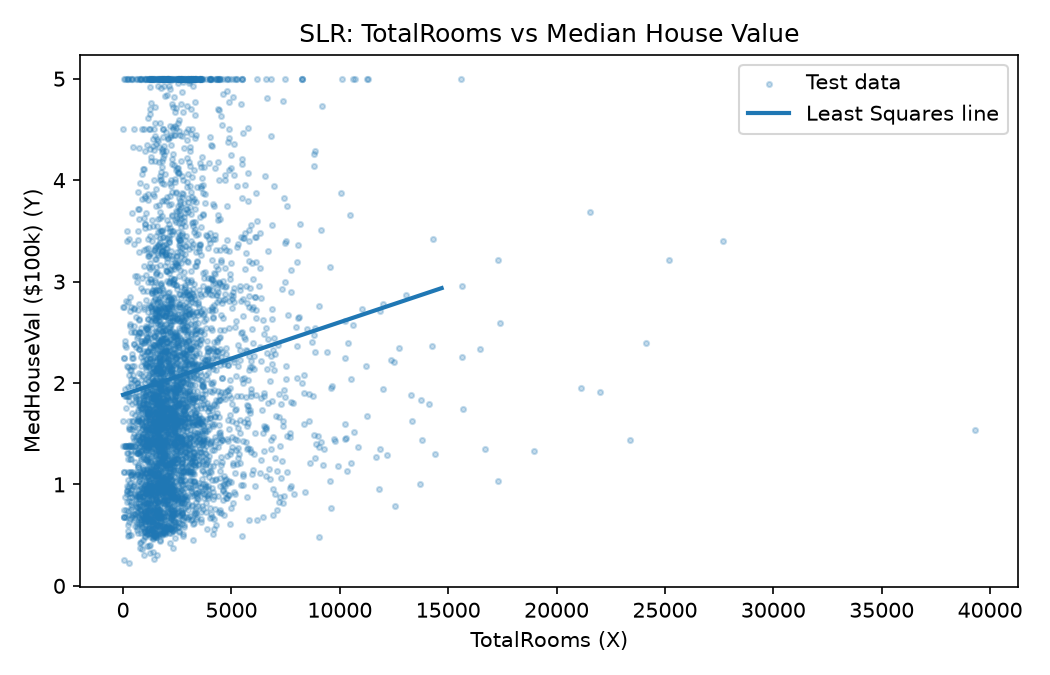
\includegraphics[width=0.78\textwidth]{exp1_ls.png}\par
\small Fig. 1: Test data with the least-squares regression line.\par
\end{center}
\vspace{4pt}

\begin{center}
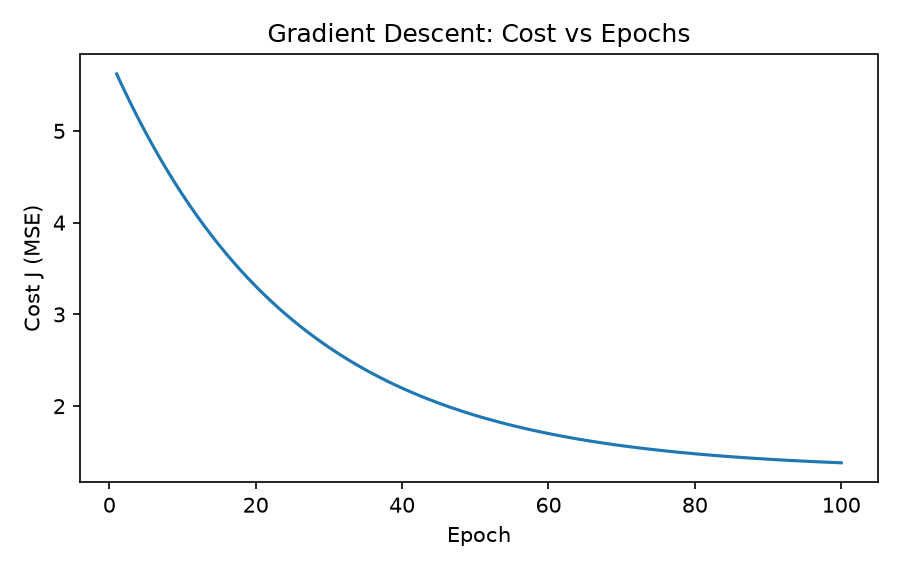
\includegraphics[width=0.62\textwidth]{exp1_cost.png}\par
\small Fig. 2: Gradient-descent cost vs epochs ($\alpha=0.01$, 100 epochs).\par
\end{center}
\vspace{4pt}

\newpage

\expheading{RESULT}
\vspace{4pt}
{\fontsize{12}{15}\selectfont
The above program was implemented and executed successfully using Python, and the corresponding output was obtained and verified. The results of the \textbf{least squares and gradient descent regression} were analyzed and found to be satisfactory, thereby achieving the desired objective of the experiment.\par
}

\vspace{12pt}

\noindent\textbf{Faculty Signature:} \underline{\hspace{3.6cm}} \hfill \textbf{Date:} \underline{\hspace{2.8cm}}\par

\end{document}
